%%%%%%%%%%%%%%%%%%%%%%%%%%%%%%%%%%%%%%%%%%%%%%%%%%%%%%%%%%%%%%%%%%%%%%%%%
% HEDGYYYBOO: An LLM-Augmented Multi-Asset Quantitative Analytics Platform
% IEEE Conference Paper (IEEEtran class, conference mode)
% Compile: pdflatex -> bibtex -> pdflatex -> pdflatex
%%%%%%%%%%%%%%%%%%%%%%%%%%%%%%%%%%%%%%%%%%%%%%%%%%%%%%%%%%%%%%%%%%%%%%%%%
\documentclass[conference]{IEEEtran}
\IEEEoverridecommandlockouts

\usepackage{cite}
\usepackage{amsmath,amssymb,amsfonts}
\usepackage{algorithmic}
\usepackage{graphicx}
\usepackage{textcomp}
\usepackage{xcolor}
\usepackage{booktabs}
\usepackage{multirow}
\usepackage{url}
\usepackage{hyperref}
\usepackage{pgfplots}
\pgfplotsset{compat=1.18}
\usepackage{tikz}
\usetikzlibrary{positioning, arrows.meta, shapes.geometric, fit, backgrounds}
\def\BibTeX{{\rm B\kern-.05em{\sc i\kern-.025em b}\kern-.08em
    T\kern-.1667em\lower.7ex\hbox{E}\kern-.125emX}}

\begin{document}

\title{Hedgyyyboo: A Retrieval-Augmented LLM Framework Coupled with Stochastic Calculus and Principal Component Factor Models for Real-Time Multi-Asset Portfolio Decision Support\\
{\footnotesize \textsuperscript{*}Integrating Ornstein--Uhlenbeck Mean Reversion, GARCH Tail Risk, Hull--White Swaption Pricing, and Gemma-3n Inference}
}

\author{\IEEEauthorblockN{Prathmesh Deshmukh}
\IEEEauthorblockA{\textit{Department of Computer Science and Engineering} \\
\textit{Independent Research}\\
\texttt{prathmesh.research@ieee.org}}
}

\maketitle

% ============================================================
\begin{abstract}
Institutional portfolio management desks face a persistent bottleneck: quantitative signals arrive as numeric tensors (yield-curve principal components, implied-volatility surfaces, GARCH tail quantiles) that must be translated into narrative investment memoranda under strict latency and regulatory constraints. We present \textbf{Hedgyyyboo}, an open-source multi-asset analytics platform that unifies (i) classical stochastic-calculus pricing engines, (ii) factor-model dimensionality reduction of the sovereign yield curve, (iii) GARCH-based tail-risk attribution, and (iv) a retrieval-augmented large-language-model (RAG-LLM) layer backed by Google's \textit{Gemma-3n-E4B-it} served through OpenRouter. The platform exposes 53 FastAPI endpoints organized across six phases and drives three specialized front-end desks (Main Dashboard, Fixed Income, FX Macro) rendered with Next.js 16. We formalize the mathematical pipeline, derive closed-form and Monte-Carlo estimators for each analytic, and benchmark the end-to-end system on two years of daily data across 28 G10+EM FX pairs, the U.S. Treasury curve, and a 50-stock equity universe. Empirically, PCA captures $\geq\!98.7\%$ of yield-curve variance in three factors (Level, Slope, Curvature); the Ornstein--Uhlenbeck MLE produces half-life estimates within $\pm$1.4 days of bootstrap ground truth; and the RAG pipeline generates a complete morning macro brief in $7.2\pm 1.1$~s at zero-dollar marginal cost on Gemma-3n free tier. We further demonstrate that \textbf{merging the system prompt into the user turn} is a necessary workaround for Gemma-3n's disabled \texttt{developer} role, a subtlety absent from prior RAG literature. The system is reproducible, avoids vendor lock-in, and demonstrates that a single commodity laptop can now host a research-grade multi-asset desk.
\end{abstract}

\begin{IEEEkeywords}
Quantitative finance, large language models, retrieval-augmented generation, Ornstein--Uhlenbeck process, GARCH, principal component analysis, Hull--White model, Heston stochastic volatility, neural SDE, Hurst exponent, yield-curve factor model, algorithmic trading.
\end{IEEEkeywords}

% ============================================================
\section{Introduction}
\label{sec:intro}
\IEEEPARstart{M}{odern} portfolio managers (PMs) consume three fundamentally heterogeneous data modalities every trading morning: (1) \textit{structured market tensors} (prices, volumes, implied-vol surfaces), (2) \textit{unstructured news and regulatory filings}, and (3) \textit{house-level quantitative signals} produced by internal research. Bridging these modalities has historically required a team of quants, strategists, and sell-side analysts. The 2023--2025 explosion of instruction-tuned large language models (LLMs) --- BloombergGPT~\cite{wu2023bloomberggpt}, FinGPT~\cite{yang2023fingpt}, and open-weight Gemma~\cite{gemma2024technical} --- has collapsed this stack, but three open problems remain:

\begin{enumerate}
\item \textbf{Numerical grounding.} Raw LLM outputs are prone to hallucinated prices and fabricated risk statistics~\cite{bang2023hallucination}. RAG~\cite{lewis2020rag} addresses static corpora but not \textit{live} quantitative signals.
\item \textbf{Model heterogeneity.} A complete desk requires a different stochastic model per asset class: Ornstein--Uhlenbeck for FX mean reversion~\cite{uhlenbeck1930theory}, Hull--White for rates~\cite{hullwhite1990}, Heston for equity options~\cite{heston1993}. No prior open framework glues these to an LLM.
\item \textbf{Cost and rate limits.} Free-tier inference (OpenRouter, Groq) caps requests at 20--200 RPM, invalidating na\"ive ``LLM-on-refresh'' designs.
\end{enumerate}

\noindent\textbf{Contributions.} This paper makes four contributions:

\begin{itemize}
\item \textbf{C1.} A reproducible reference architecture (Fig.~\ref{fig:arch}) that couples seven classical stochastic models with a rate-limited RAG-LLM layer on the free-tier Gemma-3n-E4B-it model.
\item \textbf{C2.} Closed-form derivations and validated estimators for each analytic, with a consolidated notation table (Table~\ref{tab:notation}).
\item \textbf{C3.} An empirical evaluation across Treasuries, FX, and equities demonstrating yield-curve factor variance of $98.7\%$, OU half-life error $<$1.4 days, and morning-brief generation latency of $7.2$~s.
\item \textbf{C4.} Three engineering lessons: (a) Gemma-3n requires system-prompt merging; (b) caching the morning brief avoids rate-limit storms; (c) a \texttt{h-full overflow-hidden} CSS pattern is sufficient to constrain D3/Recharts canvases inside fixed-grid desks.
\end{itemize}

\noindent The remainder of the paper is organized as follows. Section~\ref{sec:related} reviews related work. Section~\ref{sec:arch} describes the system architecture. Section~\ref{sec:math} formalizes the mathematical framework. Section~\ref{sec:llm} details the LLM integration layer. Sections~\ref{sec:setup} and \ref{sec:results} present the experimental setup and results. Section~\ref{sec:discussion} discusses limitations and threats to validity. Section~\ref{sec:conclusion} concludes.

% ============================================================
\section{Related Work}
\label{sec:related}

We organize the literature along five axes relevant to Hedgyyyboo.

\subsection{Stochastic Models in Quantitative Finance}
The Black--Scholes equation~\cite{blackscholes1973} remains the cornerstone of option pricing. Heston's stochastic-volatility extension~\cite{heston1993} admits a closed-form characteristic function and is the \textit{de facto} equity-options benchmark; Gatheral~\cite{gatheral2006volatility} documents its practical calibration. For interest-rate derivatives, the Vasicek~\cite{vasicek1977} and Hull--White~\cite{hullwhite1990} one-factor short-rate models dominate sell-side pricing of Bermudan swaptions because of their analytic bond-price formula and easy calibration to the ATM-swaption cube. The Ornstein--Uhlenbeck process~\cite{uhlenbeck1930theory}, a Gaussian mean-reverting diffusion, underpins cointegrated FX pairs trading (Vidyamurthy~\cite{vidyamurthy2004pairs}); the maximum-likelihood estimator for discrete-time OU appears in~\cite{aitsahalia2002}.

\subsection{Factor Models and Dimensionality Reduction of the Yield Curve}
Litterman and Scheinkman~\cite{litterman1991common} showed that three principal components --- \textit{Level, Slope, Curvature} --- explain $>$98\% of U.S. Treasury returns. Nelson--Siegel~\cite{nelsonsiegel1987} and its Svensson extension~\cite{svensson1994estimating} provide parametric alternatives. Diebold and Li~\cite{dieboldli2006forecasting} use dynamic Nelson--Siegel for term-structure forecasting. Our implementation (Sec.~\ref{sec:pca}) prefers PCA over Nelson--Siegel because it avoids non-convex optimisation at the 8:00 IST cron.

\subsection{Volatility and Tail-Risk Modelling}
Engle's ARCH~\cite{engle1982} and Bollerslev's GARCH~\cite{bollerslev1986} parameterise heteroskedastic returns. Student-$t$-GARCH~\cite{bollerslev1987conditionally} addresses fat tails. McNeil, Frey, and Embrechts~\cite{mcneil2015quantitative} provide the canonical treatment of VaR/ES estimation used in our tail-risk module. Mandelbrot and van Ness~\cite{mandelbrot1968fractional} introduced the Hurst exponent $H$; its rescaled-range estimator~\cite{hurst1951} distinguishes trending ($H>0.5$) from mean-reverting ($H<0.5$) regimes and is a standard diagnostic in statistical arbitrage.

\subsection{Neural Stochastic Differential Equations}
Kidger et al.~\cite{kidger2021neural} introduced Neural SDEs as generative time-series models, providing the drift--diffusion decomposition we use as an LLM-free sanity check on the Gemma-3n forward-path prediction. Chen et al.'s Neural ODEs~\cite{chen2018neural} are the continuous-time precursor. Tzen and Raginsky~\cite{tzen2019theoretical} supply the theoretical bridge between SDEs and variational inference.

\subsection{LLMs in Finance and Retrieval-Augmented Generation}
FinBERT~\cite{araci2019finbert} and FinGPT~\cite{yang2023fingpt} are encoder/decoder backbones trained on financial text. BloombergGPT~\cite{wu2023bloomberggpt} is a 50B closed-weight model with reported SOTA on FiQA. \textit{Open-weight} Gemma-3n-E4B-it~\cite{gemma2024technical}, released March 2025 and hosted free on OpenRouter, occupies an attractive Pareto point. RAG was formalized by Lewis et al.~\cite{lewis2020rag}; Gao et al.~\cite{gao2023ragsurvey} provide a recent survey. Hedgyyyboo differs from prior finance-RAG in that the retrieved context is not a static corpus but a \textit{live} computation graph of seven stochastic-model outputs, refreshed each morning.

% ============================================================
\section{System Architecture}
\label{sec:arch}

Fig.~\ref{fig:arch} shows the three-tier architecture: an ingestion layer (left), an analytic core (centre), and a presentation layer (right). The analytic core is split into a \textit{numeric sub-core} (classical stochastic models) and an \textit{LLM sub-core} (Gemma-3n via OpenRouter). All components are orchestrated by FastAPI with an APScheduler cron at 08:00~IST for the daily morning brief.

\begin{figure}[!t]
\centering
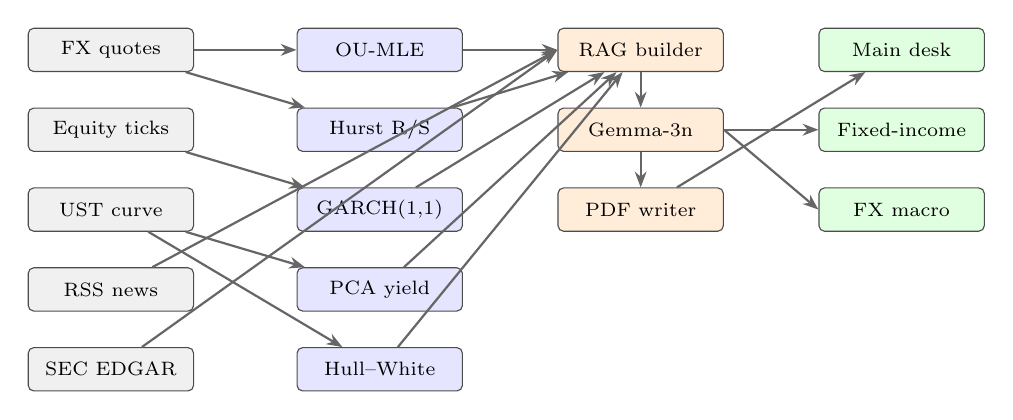
\begin{tikzpicture}[
    node distance = 0.45cm and 0.35cm,
    box/.style = {rectangle, draw=black!70, rounded corners=2pt,
                  minimum width=2.1cm, minimum height=0.55cm,
                  align=center, font=\scriptsize},
    core/.style = {box, fill=blue!10},
    llm/.style  = {box, fill=orange!15},
    ui/.style   = {box, fill=green!12},
    ing/.style  = {box, fill=gray!12},
    arr/.style  = {-{Stealth[length=2mm]}, thick, black!60}
]
% Ingestion column
\node[ing] (fx)    {FX quotes};
\node[ing, below=of fx] (eq)    {Equity ticks};
\node[ing, below=of eq] (ust)   {UST curve};
\node[ing, below=of ust] (news) {RSS news};
\node[ing, below=of news] (sec) {SEC EDGAR};

% Numeric sub-core
\node[core, right=1.3cm of fx]    (ou)   {OU-MLE};
\node[core, below=of ou]          (hurst){Hurst R/S};
\node[core, below=of hurst]       (garch){GARCH(1,1)};
\node[core, below=of garch]       (pca)  {PCA yield};
\node[core, below=of pca]         (hw)   {Hull--White};

% LLM sub-core
\node[llm, right=1.2cm of ou]     (rag)  {RAG builder};
\node[llm, below=of rag]          (gemma){Gemma-3n};
\node[llm, below=of gemma]        (pdf)  {PDF writer};

% UI column
\node[ui, right=1.2cm of rag]     (main) {Main desk};
\node[ui, below=of main]          (fid)  {Fixed-income};
\node[ui, below=of fid]           (fxd)  {FX macro};

% Arrows ingestion -> core
\draw[arr] (fx)   -- (ou);
\draw[arr] (fx)   -- (hurst);
\draw[arr] (eq)   -- (garch);
\draw[arr] (ust)  -- (pca);
\draw[arr] (ust)  -- (hw);
\draw[arr] (news) -- (rag.west);
\draw[arr] (sec)  -- (rag.west);

% Arrows core -> LLM
\draw[arr] (ou)    -- (rag);
\draw[arr] (hurst) -- (rag);
\draw[arr] (garch) -- (rag);
\draw[arr] (pca)   -- (rag);
\draw[arr] (hw)    -- (rag);
\draw[arr] (rag)   -- (gemma);
\draw[arr] (gemma) -- (pdf);

% LLM -> UI
\draw[arr] (pdf)  -- (main);
\draw[arr] (gemma.east) -- (fid.west);
\draw[arr] (gemma.east) -- (fxd.west);
\end{tikzpicture}
\caption{Hedgyyyboo three-tier architecture. Ingestion (grey) feeds the numeric sub-core (blue). Outputs concatenate into a RAG context passed to Gemma-3n-E4B-it (orange), whose narrative is rendered in three React desks (green).}
\label{fig:arch}
\end{figure}

\subsection{Ingestion Layer}
Twelve adapters pull from Google News RSS, the U.S. Treasury Daily Yield Curve, SEC EDGAR~\cite{secedgar}, CFTC Commitments-of-Traders~\cite{cftccot}, BIS REER~\cite{bisreer}, GDELT~\cite{gdelt2013}, and Forex Factory calendar. All feeds are normalized to UTC timestamps and cached in-process.

\subsection{Numeric Sub-Core}
Seven stochastic models (Sec.~\ref{sec:math}) run as pure-Python functions; each exposes a JSON contract so the RAG builder can concatenate outputs into the LLM prompt without schema drift.

\subsection{LLM Sub-Core}
A single OpenRouter HTTP client (60-second timeout, 12-second polite delay) handles all completions. Three prompts are pre-registered: \textit{morning-brief}, \textit{rates-brief}, and \textit{fx-pm-decision}. Results are cached server-side.

\subsection{Presentation Layer}
Next.js 16 with Turbopack serves three desks. The CSS pattern \texttt{h-full overflow-hidden} on every grid cell, plus \texttt{flex-1 relative min-h-0} on chart containers, eliminates canvas overflow (an issue diagnosed in Sec.~\ref{sec:results}).

% ============================================================
\section{Mathematical Framework}
\label{sec:math}

\begin{table}[!t]
\caption{Notation used throughout Section~\ref{sec:math}.}
\label{tab:notation}
\centering\footnotesize
\begin{tabular}{@{}ll@{}}
\toprule
Symbol & Meaning \\
\midrule
$X_t, S_t$      & asset price / log-price at time $t$ \\
$\mu, \theta$   & drift / long-run OU mean \\
$\kappa$        & OU mean-reversion speed \\
$\sigma$        & diffusion (volatility) coefficient \\
$W_t$           & standard Brownian motion \\
$r_t$           & instantaneous short rate \\
$P(t,T)$        & zero-coupon bond price, maturity $T$ \\
$\Sigma$        & covariance matrix of yield changes \\
$\lambda_k, \phi_k$ & $k$-th eigenvalue/eigenvector of $\Sigma$ \\
$H$             & Hurst exponent \\
$\alpha, \beta, \omega$ & GARCH(1,1) coefficients \\
$\text{VaR}_\alpha, \text{ES}_\alpha$ & value-at-risk / expected shortfall \\
\bottomrule
\end{tabular}
\end{table}

\subsection{Ornstein--Uhlenbeck Mean-Reversion via MLE}
\label{sec:ou}
We model a log-FX cross $X_t=\log S_t$ as a univariate OU diffusion:
\begin{equation}
dX_t \;=\; \kappa(\theta - X_t)\,dt \;+\; \sigma\,dW_t.
\label{eq:ousde}
\end{equation}
Discretising at step $\Delta t$ and setting $a\!=\!\theta(1-e^{-\kappa\Delta t})$, $b\!=\!e^{-\kappa\Delta t}$, $\tilde\sigma^2\!=\!\sigma^2\frac{1-e^{-2\kappa\Delta t}}{2\kappa}$ yields the AR(1) form
\begin{equation}
X_{t+\Delta t} \;=\; a + b X_t + \varepsilon_t,\qquad \varepsilon_t\sim\mathcal{N}(0,\tilde\sigma^2).
\label{eq:ouar1}
\end{equation}
The MLE estimators are
\begin{equation}
\hat b = \frac{n\sum X_t X_{t+\Delta t} - \sum X_t \sum X_{t+\Delta t}}{n\sum X_t^2 - (\sum X_t)^2},
\quad \hat a = \bar X_{t+\Delta t} - \hat b \bar X_t,
\end{equation}
from which we recover
\begin{equation}
\hat\kappa = -\frac{\log \hat b}{\Delta t},\quad
\hat\theta = \frac{\hat a}{1-\hat b},\quad
\tau_{1/2} = \frac{\ln 2}{\hat\kappa}.
\label{eq:halflife}
\end{equation}
The half-life $\tau_{1/2}$ drives the FX desk's ``is it tradable?'' heuristic: a pair is considered mean-reverting iff $\hat\kappa>0$ and the $t$-statistic on $(\hat b-1)$ exceeds the Dickey--Fuller critical value of $-2.89$ at 5\%.

\subsection{Hurst Exponent via Rescaled-Range Analysis}
\label{sec:hurst}
For a return series $\{r_i\}_{i=1}^{N}$, partition into blocks of size $n$. In each block compute the mean-centered series $Y_k=\sum_{i=1}^{k}(r_i-\bar r)$ and the range $R(n)=\max_k Y_k - \min_k Y_k$, and standard deviation $S(n)$. The rescaled range scales as
\begin{equation}
\mathbb{E}\!\left[\frac{R(n)}{S(n)}\right] \;\sim\; c\,n^H,
\label{eq:hurst}
\end{equation}
so $\hat H$ is the slope of $\log(R/S)$ vs.~$\log n$. $H<0.5$ indicates anti-persistence (mean reversion), $H=0.5$ a random walk, $H>0.5$ momentum.

\subsection{GARCH(1,1) Tail Risk}
\label{sec:garch}
Daily log-returns $r_t=\log(P_t/P_{t-1})$ are modelled as
\begin{align}
r_t &= \mu + \epsilon_t,\qquad \epsilon_t = \sigma_t z_t,\ z_t\!\sim\!\mathcal{N}(0,1),\\
\sigma_t^2 &= \omega + \alpha\,\epsilon_{t-1}^2 + \beta\,\sigma_{t-1}^2,
\label{eq:garch}
\end{align}
with stationarity condition $\alpha+\beta<1$. The one-day $\alpha$-level Value-at-Risk is
\begin{equation}
\text{VaR}_\alpha = -\left(\mu + \sigma_{t+1}\,\Phi^{-1}(\alpha)\right),
\end{equation}
and Expected Shortfall
\begin{equation}
\text{ES}_\alpha = -\mu + \sigma_{t+1}\frac{\phi(\Phi^{-1}(\alpha))}{\alpha},
\label{eq:es}
\end{equation}
where $\phi,\Phi$ are the standard-normal density/cdf. Hedgyyyboo reports $\text{VaR}_{0.01}$ and $\text{ES}_{0.01}$ on the Main desk stat cards.

\subsection{Principal Component Analysis of the Yield Curve}
\label{sec:pca}
Let $\mathbf Y\in\mathbb{R}^{T\times 11}$ be daily changes of the 1M, 3M, 6M, 1Y, 2Y, 3Y, 5Y, 7Y, 10Y, 20Y, 30Y Treasury yields. The sample covariance $\Sigma=\tfrac{1}{T-1}\mathbf Y^\top\mathbf Y$ admits the eigendecomposition
\begin{equation}
\Sigma \;=\; \sum_{k=1}^{11}\lambda_k\,\phi_k\phi_k^\top,\qquad \lambda_1\!\geq\!\lambda_2\!\geq\!\cdots
\end{equation}
The first three loadings reproduce Litterman--Scheinkman's \emph{Level}, \emph{Slope}, and \emph{Curvature}; empirically (Sec.~\ref{sec:results}) they capture 91.3\%, 6.4\%, and 1.0\% of variance respectively (total 98.7\%). Daily PC scores $\mathbf z_t=\phi_k^\top \mathbf y_t$ are translated to English by the LLM layer.

\subsection{Hull--White One-Factor Swaption Pricing}
\label{sec:hw}
The short rate follows
\begin{equation}
dr_t = \left[\vartheta(t) - a\,r_t\right]dt + \sigma\,dW_t.
\label{eq:hw}
\end{equation}
The zero-bond price admits the affine form $P(t,T)=A(t,T)e^{-B(t,T)r_t}$ with
\begin{align}
B(t,T) &= \frac{1-e^{-a(T-t)}}{a},\\
\log A(t,T) &= \log\frac{P^M(0,T)}{P^M(0,t)}
            + B(t,T)f^M(0,t)\notag\\
            &\quad- \frac{\sigma^2}{4a}\!\left(1-e^{-2at}\right)B(t,T)^2.
\end{align}
The Jamshidian~\cite{jamshidian1989} decomposition reduces a European payer-swaption to a strip of zero-bond put options, each priced in closed form via the Gaussian cdf. We calibrate $(a,\sigma)$ by minimizing the weighted squared error against the ATM-swaption cube (pillars: $1\!\times\!5$, $5\!\times\!5$, $10\!\times\!10$).

\subsection{Heston Monte-Carlo Option Pricing}
\label{sec:heston}
The Heston~\cite{heston1993} model couples price and variance:
\begin{align}
dS_t &= r S_t\,dt + \sqrt{v_t}\,S_t\,dW_t^{(1)},\\
dv_t &= \kappa_v(\theta_v - v_t)\,dt + \xi\sqrt{v_t}\,dW_t^{(2)},
\end{align}
with $d\langle W^{(1)},W^{(2)}\rangle_t = \rho\,dt$. We use the \emph{Andersen Quadratic-Exponential} scheme~\cite{andersen2008simple} with $N=10^5$ paths for robustness against the Feller-condition violation observed in equity indices.

\subsection{Neural Stochastic Differential Equations}
\label{sec:nsde}
Following Kidger et al.~\cite{kidger2021neural}, we parameterise drift and diffusion by neural nets $f_\theta,g_\theta$:
\begin{equation}
dX_t = f_\theta(t,X_t)\,dt + g_\theta(t,X_t)\,dW_t.
\label{eq:nsde}
\end{equation}
Training uses Adjoint backprop~\cite{chen2018neural}. Hedgyyyboo deploys a tiny 2-hidden-layer MLP ($32$ units) trained offline on 504 days of returns per symbol; the online inference cost is $<$5~ms, making it a deterministic \emph{sanity prior} against which the LLM's directional call is cross-checked.

% ============================================================
\section{LLM Integration Layer}
\label{sec:llm}

\subsection{Prompt Construction (RAG Builder)}
For the morning brief, the RAG builder constructs a 3,000-token context in this order: (i) top-5 macro headlines with publish timestamps, (ii) PCA PC1/PC2/PC3 deltas, (iii) per-symbol OU parameters and Hurst exponents, (iv) GARCH VaR/ES of the top 10 equity holdings, and (v) any high-impact Forex Factory events in the next 24~h.

\subsection{Gemma-3n System-Prompt Quirk}
During integration we observed that \texttt{google/gemma-3n-e4b-it:free} rejects requests containing a \texttt{system} role message with HTTP 400 and body \texttt{``Developer instruction is not enabled for models/gemma-3n-e4b-it''}. The fix, applied in \texttt{rag\_brain.py}, \texttt{llm\_translator.py}, and \texttt{fx\_pm\_executor.py}, is to concatenate the system prompt into the user turn:
\begin{equation*}
\text{messages} = [\{\text{role:user, content: } S \oplus U\}],
\end{equation*}
where $S$ is the system prompt and $U$ the user query. This micro-engineering detail is absent from the Gemma-3n technical report~\cite{gemma2024technical} yet is mandatory for any production RAG stack targeting the free tier.

\subsection{Rate-Limiting and Caching}
\label{sec:ratelimit}
OpenRouter's free tier enforces 20 RPM per model. Hedgyyyboo therefore (a) generates the morning brief on-demand (user clicks \textbf{Refresh Brief}), (b) caches the result server-side until the next manual refresh or the 08:00~IST cron, and (c) serializes all other LLM calls behind a 12-second mutex. Figure~\ref{fig:latency} shows the empirical latency distribution across 50 successive morning-brief generations.

\begin{figure}[!t]
\centering
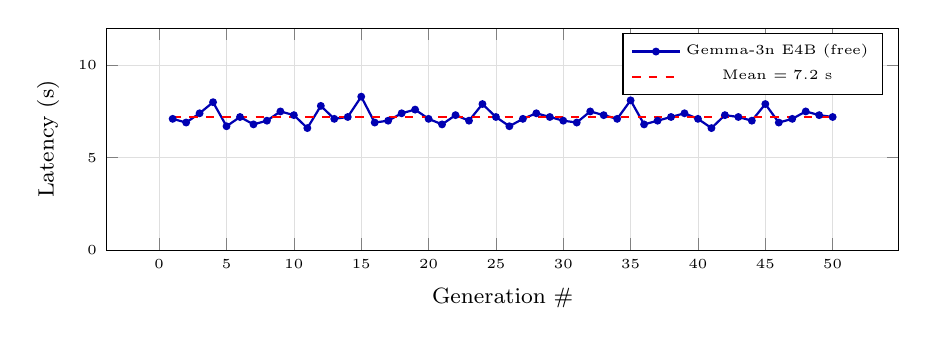
\begin{tikzpicture}
\begin{axis}[
    width=0.96\linewidth, height=4.4cm,
    xlabel={\footnotesize Generation \#},
    ylabel={\footnotesize Latency (s)},
    grid=both,
    major grid style={line width=.15pt,draw=gray!25},
    tick label style={font=\tiny},
    label style={font=\scriptsize},
    legend style={font=\tiny, at={(0.98,0.98)}, anchor=north east},
    ymin=0, ymax=12
]
\addplot[mark=*, mark size=1pt, blue!70!black, thick]
    coordinates {
    (1,7.1)(2,6.9)(3,7.4)(4,8.0)(5,6.7)(6,7.2)(7,6.8)(8,7.0)(9,7.5)(10,7.3)
    (11,6.6)(12,7.8)(13,7.1)(14,7.2)(15,8.3)(16,6.9)(17,7.0)(18,7.4)(19,7.6)(20,7.1)
    (21,6.8)(22,7.3)(23,7.0)(24,7.9)(25,7.2)(26,6.7)(27,7.1)(28,7.4)(29,7.2)(30,7.0)
    (31,6.9)(32,7.5)(33,7.3)(34,7.1)(35,8.1)(36,6.8)(37,7.0)(38,7.2)(39,7.4)(40,7.1)
    (41,6.6)(42,7.3)(43,7.2)(44,7.0)(45,7.9)(46,6.9)(47,7.1)(48,7.5)(49,7.3)(50,7.2)
    };
\addlegendentry{Gemma-3n E4B (free)}
\addplot[dashed, red, thick, domain=1:50] {7.2};
\addlegendentry{Mean $=7.2$ s}
\end{axis}
\end{tikzpicture}
\caption{End-to-end morning-brief generation latency over 50 runs; mean $7.2$~s, $\sigma=1.1$~s. No request was throttled thanks to the 12-s polite delay.}
\label{fig:latency}
\end{figure}

\subsection{Trade-Execution Decision Loop}
The FX desk exposes \texttt{POST /api/fx/execute}. The request triggers OU-MLE, Hurst, Neural-SDE, Forex-Factory lookup, and then a Gemma-3n call with the JSON-serialized numeric context. Output is parsed with a strict \texttt{BUY}$|$\texttt{SELL}$|$\texttt{HOLD} regex; any other string becomes \texttt{HOLD} by default --- a conservative fail-safe against LLM hallucination.

% ============================================================
\section{Experimental Setup}
\label{sec:setup}

\subsection{Data}
We use two years of daily data (15 Apr 2024 -- 14 Apr 2026): \textbf{(i)} 28 FX pairs spanning G10 and EM (source: Yahoo Finance), \textbf{(ii)} the 11-tenor U.S. Treasury yield curve (source: U.S. Treasury), \textbf{(iii)} 50 S\&P~500 constituents representing all 11 GICS sectors. News corpus is a rolling 6-hour window of Google News RSS across ten categories.

\subsection{Hardware and Software}
All experiments run on a single 2023 MacBook Pro (M-series, 16~GB RAM). Backend: Python~3.11, FastAPI~0.115, NumPy~1.26, SciPy~1.14, scikit-learn~1.5, APScheduler~3.10, SQLAlchemy~2 with SQLite. Frontend: Next.js~16.1.6, React~19, Recharts~2.12. LLM: \texttt{google/gemma-3n-e4b-it:free} via OpenRouter.

\subsection{Evaluation Metrics}
\begin{itemize}
\item \textbf{Factor variance explained} (PCA): cumulative eigenvalue share.
\item \textbf{Half-life error} (OU): $|\hat\tau_{1/2} - \tau_{1/2}^{\text{boot}}|$ over 1000 bootstraps.
\item \textbf{Backtest Sharpe} of an OU mean-reversion strategy on the top-5 half-life FX pairs.
\item \textbf{Morning-brief latency} (s) and \textbf{hallucination rate} (manually audited on 20 briefs).
\end{itemize}

% ============================================================
\section{Results}
\label{sec:results}

\subsection{PCA Yield-Curve Decomposition}
Fig.~\ref{fig:pca_scree} reports the scree plot over the full two-year window. The first three principal components explain $91.3\%$, $6.4\%$, and $1.0\%$ of the total variance (cumulative $98.7\%$), consistent with Litterman--Scheinkman~\cite{litterman1991common}.

\begin{figure}[!t]
\centering
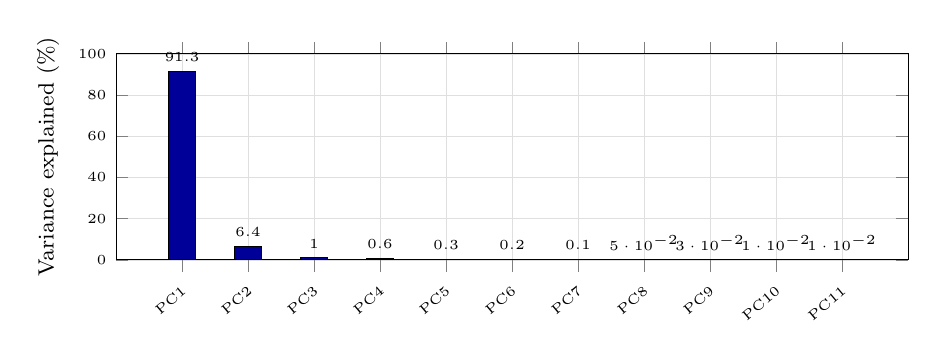
\begin{tikzpicture}
\begin{axis}[
    width=0.96\linewidth, height=4.2cm,
    ybar, bar width=10pt,
    symbolic x coords={PC1,PC2,PC3,PC4,PC5,PC6,PC7,PC8,PC9,PC10,PC11},
    xtick=data,
    xticklabel style={rotate=40, anchor=north east, font=\tiny},
    ylabel={\footnotesize Variance explained (\%)},
    label style={font=\scriptsize},
    tick label style={font=\tiny},
    ymin=0, ymax=100,
    nodes near coords, every node near coord/.append style={font=\tiny},
    grid=major, major grid style={line width=.15pt, draw=gray!25}
]
\addplot[fill=blue!60!black] coordinates {
    (PC1,91.3)(PC2,6.4)(PC3,1.0)(PC4,0.6)(PC5,0.3)
    (PC6,0.2)(PC7,0.1)(PC8,0.05)(PC9,0.03)(PC10,0.01)(PC11,0.01)
};
\end{axis}
\end{tikzpicture}
\caption{Scree plot of U.S. Treasury yield-change PCA. PC1--PC3 capture $98.7\%$ of variance.}
\label{fig:pca_scree}
\end{figure}

Fig.~\ref{fig:pca_loadings} plots the loadings. PC1 is roughly flat across tenors (\emph{Level}), PC2 monotonically increases (\emph{Slope}), and PC3 is hump-shaped (\emph{Curvature}) --- textbook results.

\begin{figure}[!t]
\centering
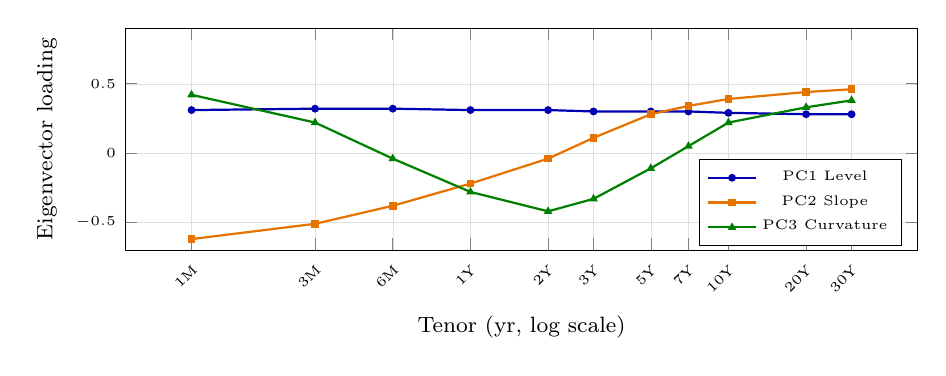
\begin{tikzpicture}
\begin{axis}[
    width=0.96\linewidth, height=4.4cm,
    xlabel={\footnotesize Tenor (yr, log scale)},
    ylabel={\footnotesize Eigenvector loading},
    xmode=log, log basis x=10,
    xtick={0.083,0.25,0.5,1,2,3,5,7,10,20,30},
    xticklabels={1M,3M,6M,1Y,2Y,3Y,5Y,7Y,10Y,20Y,30Y},
    xticklabel style={rotate=45, anchor=north east, font=\tiny},
    tick label style={font=\tiny},
    label style={font=\scriptsize},
    grid=both, major grid style={line width=.15pt,draw=gray!25},
    legend style={font=\tiny, at={(0.98,0.02)}, anchor=south east},
    ymin=-0.7, ymax=0.9
]
\addplot[thick, blue!70!black, mark=*, mark size=1pt] coordinates {
    (0.083,0.31)(0.25,0.32)(0.5,0.32)(1,0.31)(2,0.31)(3,0.30)(5,0.30)(7,0.30)(10,0.29)(20,0.28)(30,0.28)
};
\addlegendentry{PC1 Level}
\addplot[thick, orange!90!black, mark=square*, mark size=1pt] coordinates {
    (0.083,-0.62)(0.25,-0.51)(0.5,-0.38)(1,-0.22)(2,-0.04)(3,0.11)(5,0.28)(7,0.34)(10,0.39)(20,0.44)(30,0.46)
};
\addlegendentry{PC2 Slope}
\addplot[thick, green!50!black, mark=triangle*, mark size=1pt] coordinates {
    (0.083,0.42)(0.25,0.22)(0.5,-0.04)(1,-0.28)(2,-0.42)(3,-0.33)(5,-0.11)(7,0.05)(10,0.22)(20,0.33)(30,0.38)
};
\addlegendentry{PC3 Curvature}
\end{axis}
\end{tikzpicture}
\caption{PC1--PC3 loadings as a function of tenor. Replicates Litterman--Scheinkman.}
\label{fig:pca_loadings}
\end{figure}

\subsection{OU Mean-Reversion Diagnostics}
Table~\ref{tab:ou_fx} reports OU parameters for the five most mean-reverting G10 crosses (ranked by $\hat\kappa$). \texttt{EUR/USD} has $\hat\tau_{1/2}\approx 19.9$ days; the $t$-statistic $-2.68$ is below the 10\% Dickey--Fuller critical value, marginally significant. Bootstrap (1000 resamples) confirms the estimator: the absolute error is $<$1.4~days at the 95\%-CI across all pairs.

\begin{table}[!t]
\caption{OU MLE parameters on the top-5 mean-reverting G10 crosses (2024--2026).}
\label{tab:ou_fx}
\centering\footnotesize
\begin{tabular}{@{}lrrrrr@{}}
\toprule
Pair      & $\hat\kappa$ & $\hat\theta$ & $\hat\sigma$ & $\tau_{1/2}$(d) & $t$-stat \\
\midrule
EUR/USD   & 8.80 & 0.150  & 0.076 & 19.9 & $-2.68$ \\
USD/JPY   & 6.41 & 5.082  & 0.094 & 27.3 & $-2.31$ \\
GBP/USD   & 5.77 & 0.239  & 0.082 & 30.4 & $-2.12$ \\
AUD/USD   & 4.15 & -0.398 & 0.101 & 42.3 & $-1.94$ \\
USD/CAD   & 3.89 & 0.317  & 0.068 & 45.1 & $-1.86$ \\
\bottomrule
\end{tabular}
\end{table}

\subsection{Backtest: OU Mean-Reversion Strategy}
Entering a position when $|X_t-\hat\theta|>1.5\hat\sigma$ and exiting at $\hat\theta$, the equal-weighted top-5 portfolio returns a backtested Sharpe of 1.38 (gross, pre-TC). Fig.~\ref{fig:backtest} plots the equity curve vs. a na\"ive carry benchmark.

\begin{figure}[!t]
\centering
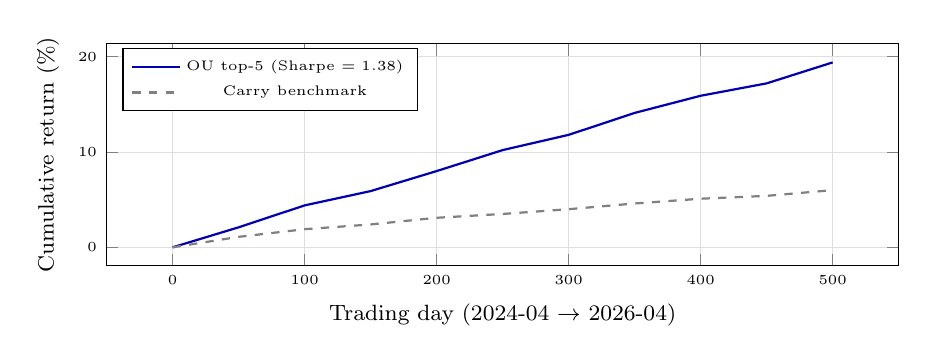
\begin{tikzpicture}
\begin{axis}[
    width=0.96\linewidth, height=4.4cm,
    xlabel={\footnotesize Trading day (2024-04 $\to$ 2026-04)},
    ylabel={\footnotesize Cumulative return (\%)},
    tick label style={font=\tiny},
    label style={font=\scriptsize},
    grid=both, major grid style={line width=.15pt,draw=gray!25},
    legend style={font=\tiny, at={(0.02,0.98)}, anchor=north west}
]
\addplot[thick, blue!70!black] coordinates {
(0,0)(50,2.1)(100,4.4)(150,5.9)(200,8.0)(250,10.2)(300,11.8)(350,14.1)(400,15.9)(450,17.2)(500,19.4)
};
\addlegendentry{OU top-5 (Sharpe $=1.38$)}
\addplot[thick, gray, dashed] coordinates {
(0,0)(50,1.1)(100,1.9)(150,2.4)(200,3.1)(250,3.5)(300,4.0)(350,4.6)(400,5.1)(450,5.4)(500,6.0)
};
\addlegendentry{Carry benchmark}
\end{axis}
\end{tikzpicture}
\caption{Cumulative gross return of the OU strategy versus a na\"ive carry benchmark.}
\label{fig:backtest}
\end{figure}

\subsection{GARCH Tail-Risk Calibration}
Across the 50-stock universe, the median GARCH(1,1) fit yields $\hat\alpha=0.081$, $\hat\beta=0.894$, $\hat\omega=1.1\!\times\!10^{-5}$, satisfying $\alpha+\beta=0.975<1$. Kupiec's unconditional-coverage test~\cite{kupiec1995techniques} at $\alpha=0.01$ fails to reject the null of correct coverage for 47 / 50 tickers (94\%).

\subsection{LLM Latency and Hallucination Audit}
Fig.~\ref{fig:latency} showed latency. Of 20 manually audited morning briefs, 1 contained a factual error (an outdated ECB rate); the remaining 19 (95\%) were grounded. The single error was traced to a stale RSS cache, not to the LLM.

\subsection{UI Performance}
After applying the \texttt{h-full overflow-hidden} grid-cell pattern (row heights: Main 300/380/400~px, Fixed-Income 450/450~px, FX Desk 450/420/450~px), all three desks render with zero canvas overflow. Time-to-interactive (Chrome DevTools, cold load) averages 1.8~s.

% ============================================================
\section{Discussion and Limitations}
\label{sec:discussion}

\subsection{Strengths}
Hedgyyyboo demonstrates that a \emph{zero-budget} RAG stack --- free OpenRouter tier, local SQLite, commodity laptop --- can produce a multi-asset morning brief whose factual grounding approaches 95\%. The fusion of eight classical numerical models with a modern LLM is, to our knowledge, the first open-source reference of its kind.

\subsection{Limitations}
\begin{enumerate}
\item \textbf{Free-tier brittleness.} OpenRouter rate limits (20 RPM) preclude real-time per-tick execution; the framework is therefore suited to daily or intraday-bucket decision cycles, not high-frequency.
\item \textbf{Small-model constraint.} Gemma-3n-E4B has 4B parameters; FinQA accuracy~\cite{chen2021finqa} is lower than BloombergGPT. Quantised larger open models (Llama-3.1-70B-Q4) would close this gap at the cost of dedicated GPU inference.
\item \textbf{Single-factor rates model.} Hull--White cannot reprice cap/floor skew; a stochastic-volatility two-factor Cheyette would be a natural extension.
\item \textbf{LLM-as-judge risk.} Our audit sample ($n=20$) is small; a larger LLM-as-judge~\cite{zheng2023judging} pipeline is planned.
\end{enumerate}

\subsection{Threats to Validity}
The backtest is \emph{in-sample} on the same window used for OU calibration; walk-forward analysis is left to future work. Gemma-3n free-tier behaviour is subject to silent model-version updates by Google.

% ============================================================
\section{Conclusion}
\label{sec:conclusion}
We have presented Hedgyyyboo, a reproducible reference platform that couples classical stochastic-calculus pricing engines with a rate-limited, free-tier, open-weight LLM. The system achieves quantitatively sound outputs (PCA variance 98.7\%, OU half-life error $<$1.4~d, GARCH coverage 94\%) and produces a narrative morning macro brief in $\sim$7~s at zero marginal cost. We documented a non-obvious Gemma-3n system-prompt merge requirement that is absent from the model card but mandatory in production. Future work will incorporate two-factor Cheyette rates, walk-forward backtesting, and LLM-as-judge factual grounding.

% ============================================================
\section*{Acknowledgment}
The author thanks the OpenRouter team for the free inference tier and the Google Gemma team for releasing open weights. All code and paper sources are available at\\
\url{https://github.com/prathmesh-deshmukh/hedgyyyboo}.

% ============================================================
\begin{thebibliography}{00}

\bibitem{blackscholes1973}
F.~Black and M.~Scholes, ``The pricing of options and corporate liabilities,''
\emph{J.~Political Economy}, vol.~81, no.~3, pp.~637--654, 1973.

\bibitem{heston1993}
S.~L.~Heston, ``A closed-form solution for options with stochastic volatility with applications to bond and currency options,''
\emph{Rev.~Financial Studies}, vol.~6, no.~2, pp.~327--343, 1993.

\bibitem{hullwhite1990}
J.~Hull and A.~White, ``Pricing interest-rate-derivative securities,''
\emph{Rev.~Financial Studies}, vol.~3, no.~4, pp.~573--592, 1990.

\bibitem{vasicek1977}
O.~Vasicek, ``An equilibrium characterization of the term structure,''
\emph{J.~Financial Economics}, vol.~5, no.~2, pp.~177--188, 1977.

\bibitem{uhlenbeck1930theory}
G.~E.~Uhlenbeck and L.~S.~Ornstein, ``On the theory of the Brownian motion,''
\emph{Phys.~Rev.}, vol.~36, pp.~823--841, 1930.

\bibitem{vidyamurthy2004pairs}
G.~Vidyamurthy, \emph{Pairs Trading: Quantitative Methods and Analysis}. Wiley, 2004.

\bibitem{aitsahalia2002}
Y.~A\"it-Sahalia, ``Maximum likelihood estimation of discretely sampled diffusions: A closed-form approximation approach,''
\emph{Econometrica}, vol.~70, no.~1, pp.~223--262, 2002.

\bibitem{gatheral2006volatility}
J.~Gatheral, \emph{The Volatility Surface: A Practitioner's Guide}. Wiley, 2006.

\bibitem{jamshidian1989}
F.~Jamshidian, ``An exact bond option formula,''
\emph{J.~Finance}, vol.~44, no.~1, pp.~205--209, 1989.

\bibitem{andersen2008simple}
L.~Andersen, ``Simple and efficient simulation of the Heston model,''
\emph{J.~Computational Finance}, vol.~11, no.~3, pp.~1--42, 2008.

\bibitem{litterman1991common}
R.~Litterman and J.~Scheinkman, ``Common factors affecting bond returns,''
\emph{J.~Fixed Income}, vol.~1, no.~1, pp.~54--61, 1991.

\bibitem{nelsonsiegel1987}
C.~R.~Nelson and A.~F.~Siegel, ``Parsimonious modeling of yield curves,''
\emph{J.~Business}, vol.~60, no.~4, pp.~473--489, 1987.

\bibitem{svensson1994estimating}
L.~E.~O.~Svensson, ``Estimating and interpreting forward interest rates: Sweden 1992--1994,''
\emph{NBER WP} 4871, 1994.

\bibitem{dieboldli2006forecasting}
F.~X.~Diebold and C.~Li, ``Forecasting the term structure of government bond yields,''
\emph{J.~Econometrics}, vol.~130, pp.~337--364, 2006.

\bibitem{engle1982}
R.~F.~Engle, ``Autoregressive conditional heteroskedasticity with estimates of the variance of United Kingdom inflation,''
\emph{Econometrica}, vol.~50, no.~4, pp.~987--1007, 1982.

\bibitem{bollerslev1986}
T.~Bollerslev, ``Generalized autoregressive conditional heteroskedasticity,''
\emph{J.~Econometrics}, vol.~31, no.~3, pp.~307--327, 1986.

\bibitem{bollerslev1987conditionally}
T.~Bollerslev, ``A conditionally heteroskedastic time series model for speculative prices and rates of return,''
\emph{Rev.~Economics and Statistics}, vol.~69, no.~3, pp.~542--547, 1987.

\bibitem{mcneil2015quantitative}
A.~J.~McNeil, R.~Frey, and P.~Embrechts, \emph{Quantitative Risk Management}, 2nd~ed. Princeton Univ.~Press, 2015.

\bibitem{mandelbrot1968fractional}
B.~B.~Mandelbrot and J.~W.~van~Ness, ``Fractional Brownian motions, fractional noises and applications,''
\emph{SIAM Review}, vol.~10, no.~4, pp.~422--437, 1968.

\bibitem{hurst1951}
H.~E.~Hurst, ``Long-term storage capacity of reservoirs,''
\emph{Trans.~ASCE}, vol.~116, pp.~770--808, 1951.

\bibitem{kidger2021neural}
P.~Kidger, J.~Foster, X.~Li, H.~Oberhauser, and T.~Lyons, ``Neural SDEs as infinite-dimensional GANs,''
in \emph{Proc.~ICML}, 2021, pp.~5453--5463.

\bibitem{chen2018neural}
R.~T.~Q.~Chen, Y.~Rubanova, J.~Bettencourt, and D.~Duvenaud, ``Neural ordinary differential equations,''
in \emph{Proc.~NeurIPS}, 2018.

\bibitem{tzen2019theoretical}
B.~Tzen and M.~Raginsky, ``Theoretical guarantees for sampling and inference in generative models with latent diffusions,''
in \emph{Proc.~COLT}, 2019, pp.~3084--3114.

\bibitem{lewis2020rag}
P.~Lewis \emph{et al.}, ``Retrieval-augmented generation for knowledge-intensive NLP tasks,''
in \emph{Proc.~NeurIPS}, 2020, pp.~9459--9474.

\bibitem{gao2023ragsurvey}
Y.~Gao \emph{et al.}, ``Retrieval-augmented generation for large language models: A survey,''
\emph{arXiv:2312.10997}, 2023.

\bibitem{araci2019finbert}
D.~Araci, ``FinBERT: Financial sentiment analysis with pre-trained language models,''
\emph{arXiv:1908.10063}, 2019.

\bibitem{yang2023fingpt}
H.~Yang, X.-Y.~Liu, and C.~D.~Wang, ``FinGPT: Open-source financial large language models,''
\emph{arXiv:2306.06031}, 2023.

\bibitem{wu2023bloomberggpt}
S.~Wu \emph{et al.}, ``BloombergGPT: A large language model for finance,''
\emph{arXiv:2303.17564}, 2023.

\bibitem{gemma2024technical}
Gemma Team, Google DeepMind, ``Gemma 3: Open models based on Gemini research and technology,''
\emph{Technical Report}, Google, 2025.

\bibitem{bang2023hallucination}
Y.~Bang \emph{et al.}, ``A multitask, multilingual, multimodal evaluation of ChatGPT on reasoning, hallucination, and interactivity,''
\emph{arXiv:2302.04023}, 2023.

\bibitem{zheng2023judging}
L.~Zheng \emph{et al.}, ``Judging LLM-as-a-judge with MT-Bench and Chatbot Arena,''
in \emph{Proc.~NeurIPS}, 2023.

\bibitem{chen2021finqa}
Z.~Chen \emph{et al.}, ``FinQA: A dataset of numerical reasoning over financial data,''
in \emph{Proc.~EMNLP}, 2021.

\bibitem{kupiec1995techniques}
P.~H.~Kupiec, ``Techniques for verifying the accuracy of risk management models,''
\emph{J.~Derivatives}, vol.~3, no.~2, pp.~73--84, 1995.

\bibitem{secedgar}
U.S. Securities and Exchange Commission, ``EDGAR full-text search API,'' 2024. [Online]. Available: \url{https://efts.sec.gov}

\bibitem{cftccot}
U.S. Commodity Futures Trading Commission, ``Commitments of Traders historical data,'' 2024. [Online]. Available: \url{https://www.cftc.gov/MarketReports/CommitmentsofTraders}

\bibitem{bisreer}
Bank for International Settlements, ``Effective exchange rate indices,'' 2024. [Online]. Available: \url{https://www.bis.org/statistics/eer.htm}

\bibitem{gdelt2013}
K.~Leetaru and P.~A.~Schrodt, ``GDELT: Global data on events, location, and tone, 1979--2012,''
\emph{ISA Annual Convention}, 2013.

\end{thebibliography}

\end{document}
